\chapter{KalSea: Kalman-Corrected Spectral-Evolution-Aware Caching}\label{ch:kalsea}

ReSPect forecasts the skipped residuals better than reuse, but like every filler in the literature it is \emph{open loop}: once the next computed step reveals how wrong the forecast was, that error has already been integrated into the latent and is never corrected. This chapter presents KalSea (\textbf{Kal}man + \textbf{SEA}), the second method of the project, which closes this loop. Behind the unchanged SEA gate of SeaCache, a damped-trend Kalman filter forecasts the block-stack residual on skipped steps (the \emph{predictor}). When the next step is computed, a Rauch--Tung--Striebel smoother turns the filter's innovation into corrected residuals for the whole skipped gap, the gap is re-integrated through the output layers only, and sampling continues from the corrected latent (the \emph{corrector}). We call this procedure predictor--corrector gap smoothing (PCGS). PCGS requires no additional transformer evaluations and no hyper-parameters of its own.

On FLUX.1-dev and held-out DrawBench prompts, KalSea reaches a PSNR of 27.72\,dB with respect to the 50-step sampler at 18.1 of 50 transformer evaluations, against 26.29\,dB reported for SeaCache at 18.4, and 22.53 against 21.33\,dB at 13 evaluations. In paired comparisons PCGS alone contributes 0.81\,dB (95\% CI $[0.63,1.00]$) and 0.61\,dB $[0.48,0.76]$, and it also improves plain reuse and linear extrapolation. On HunyuanVideo and Wan2.1 at SeaCache's budgets, KalSea improves PSNR over SeaCache run in the same setup by 1.9--3.2\,dB and 0.3--2.3\,dB.

\begin{figure}[t]
  \centering
  
\includegraphics[width=0.95\textwidth]{kalsea_teaser.pdf}
  \caption[Images generated with KalSea on FLUX.1-dev]{Images generated by FLUX.1-dev ($1024\times1024$, 50 steps) with KalSea at $\delta=0.2$, i.e.\ 27 of 50 transformer evaluations ($1.85\times$ fewer). The tiles are only downscaled; the billboard is the central 2:1 band of its image.}
  \label{fig:kalsea-teaser}
\end{figure}

%% ------------------------------------------------------------------------------------------------
\section{From ReSPect to KalSea: the open-loop problem}\label{sec:kalsea-motivation}

Reuse and forecasting share a structural limitation. The filler predicts the skipped steps from the past alone, and the sampler integrates its errors into the latent (\cref{sec:bg-residual}). These errors grow with the distance to the last computed step: on six reference trajectories of our development set, the relative error of the velocity obtained from a Kalman forecast of the residual grows from 4--5\% at the first skipped step to over 20\% at the seventh. When the next step is computed, its block-stack output reveals how wrong the forecast was, but existing caches, including ReSPect, use this observation only to predict the \emph{next} gap; the latent, already advanced along erroneous velocities, is never revisited. Forecasting reduces the drift but does not remove it, and as gaps grow its advantage over reuse vanishes (\cref{sec:kalsea-results}).

Our key observation is that \emph{a skipped gap is a smoothing problem}. With a Kalman filter as the predictor of the block-stack residual, the innovation at the next computed step $b$ (observed minus forecast residual) and the covariances accumulated over the gap determine, through the Rauch--Tung--Striebel (RTS) smoother \citep{rauch1965rts}, the minimum-mean-square-error residuals of all skipped steps under the filter's model. Because only the cheap output layers depend on the residual, the gap can be re-integrated through them and sampling can continue from the corrected latent. Like the corrector of UniPC \citep{zhao2023unipc}, PCGS reuses a network evaluation that the sampler performs anyway; unlike it, it corrects an entire gap of steps whose network outputs were never computed. The regression forecaster of ReSPect does not provide the covariances needed for such a correction, which is why KalSea moves to a state-space model.

\Cref{fig:kalsea-overview} gives an overview of the method. The gate is the SEA gate of \cref{sec:bg-sea}, used unchanged with $\beta=2$ for images and $\beta=3$ for videos; KalSea changes only what is written on the steps it skips and then corrects it.

\begin{figure}[t]
  \centering
  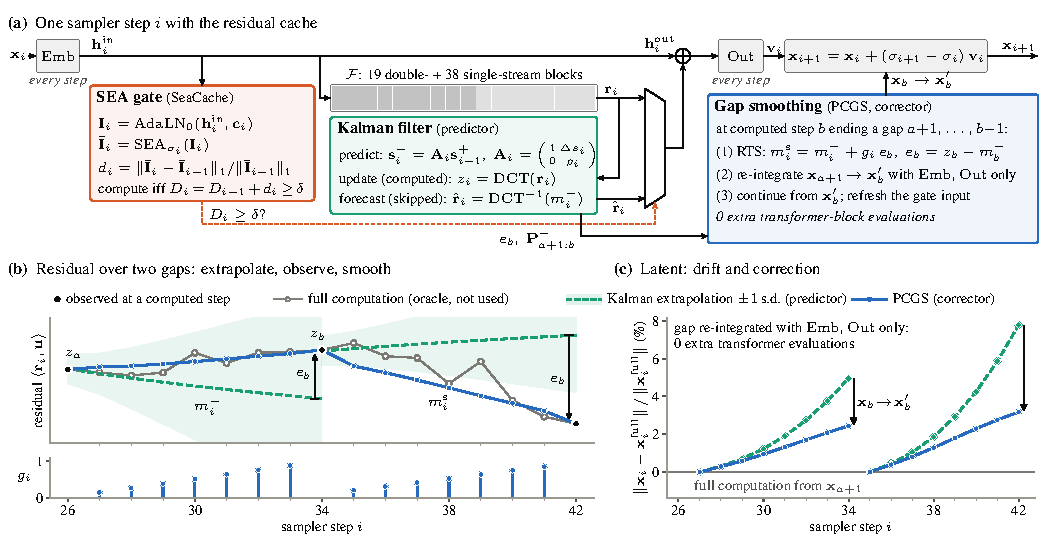
\includegraphics[width=\textwidth]{kalsea_overview.pdf}
  \caption[Overview of KalSea]{Overview of KalSea. (a) In each step the SEA gate accumulates the filtered relative change of the first block's modulated input and runs the blocks $F$ only when the sum reaches $\delta$; the residual of a computed step updates a damped-trend Kalman filter (the predictor), whose forecast replaces it on skipped steps. (b) When a computed step $b$ ends the gap $a{+}1,\dots,b{-}1$, PCGS spreads the innovation $e_b$ over the gap with RTS gains $g_i$ that grow towards $b$. (c) Re-integrating the gap from $x_{a+1}$ with $\Emb$ and $\Out$ only lowers the latent deviation from full computation at $b$ (by 25--59\% in all ten gaps of this FLUX.1-dev sample at $\delta=0.6$), without extra transformer evaluations. In (b, c) the residual is projected onto a fixed random direction in the lowest DCT band; grey: full computation, evaluated only for the figure.}
  \label{fig:kalsea-overview}
\end{figure}

%% ------------------------------------------------------------------------------------------------
\section{The Kalman residual forecaster (predictor)}\label{sec:kalsea-predictor}

\subsection{State-space model}
The residual evolves smoothly but nonlinearly along the trajectory, and the cache observes it only at the irregular steps chosen by the gate. Following the state-space model of the contemporaneous SpecKCast \citep{rajabi2026speckcast}, which forecasts the model output, we model every element of the residual as a damped trend observed in noise. The state $s_i=[m_i,\nu_i]\tr$ holds a value and its rate of change with respect to a time coordinate $s$ that increases monotonically along the schedule, with steps $\Delta s_i = s(i)-s(i-1)$. At \emph{every} step, computed or skipped, the filter predicts
\begin{equation}\label{eq:kalsea-predict}
  s^-_i = A_i\, s^+_{i-1}, \qquad P^-_i = A_i P^+_{i-1}A_i\tr + Q_i,
\end{equation}
\begin{equation}\label{eq:kalsea-AQ}
  A_i = \begin{bmatrix} 1 & \Delta s_i \\ 0 & \rho_i\end{bmatrix}, \qquad
  Q_i = q\kappa\begin{bmatrix} \Delta s_i^3/3 & \Delta s_i^2/2 \\ \Delta s_i^2/2 & \Delta s_i\end{bmatrix}, \qquad \rho_i = e^{-\Delta s_i/\tau}.
\end{equation}
$Q_i$ is the process noise of an integrated Wiener process \citep{barshalom2001estimation} with intensity $q\kappa$, and $\rho_i$ damps the trend so that forecasts over long gaps do not overshoot \citep{gardner1985damped}. Because the filter is predicted at every step and the gate's irregular schedule enters only through which steps are corrected, any pattern of computed and skipped steps is handled consistently.

On a computed step $b$ the filter observes the residual element $z_b$ with noise variance $R$ and updates, with $h=[1,0]\tr$,
\begin{equation}\label{eq:kalsea-update}
  e_b = z_b - m^-_b,\quad S_b = [P^-_b]_{00}+R,\quad k_b = P^-_b h/S_b,\quad s^+_b = s^-_b + k_b e_b,\quad P^+_b = (I-k_bh\tr)P^-_b .
\end{equation}
On skipped steps the moments are not updated ($s^+_i=s^-_i$, $P^+_i=P^-_i$) and the cache writes the predicted value, $\hat r_i = m^-_i$, into $h^{\mathrm{out}}_i = h^{\mathrm{in}}_i + \hat r_i$; the output layers run as usual. The intensity $\kappa$ is adapted online so that the mean squared innovation matches its predicted variance $S_b$ \citep{mehra1972adaptive}. In the implementation, the multiplicative factor is updated by $g^{0.2}$ with $g$ the ratio of measured to predicted innovation power, clipped to $[0.1,10]$.

\subsection{Parametrisations}
The covariance $P$ is shared by all elements (\emph{per-element} variant) or by all coefficients of a frequency band (\emph{DCT} variant), so the filter costs a few element-wise operations per step and its gains are scalars per band. All filter statistics are kept in relative units, i.e.\ the residual is divided by the square root of its (band) power, estimated from the first observation in the calibration-free mode.
\begin{itemize}
  \item \textbf{DCT variant} (default for FLUX.1-dev, following SpecKCast). The residual of each channel is laid out on the $64\times64$ token grid and transformed with an orthonormal 2D DCT; the coefficients are grouped into seven radial frequency bands, each with its own covariance and its own warped time coordinate (a band-specific sigmoid warp of the log signal-to-noise ratio of the schedule). Noise intensities, initial trend variances and band powers are calibrated once per model from 16 uncached trajectories of prompts disjoint from all evaluation prompts (the file \texttt{kalsea\_calib\_flux.json}).
  \item \textbf{Per-element variant.} One filter per element with a single shared covariance; the time coordinate is a warped log-SNR or simply the step index. With the step index and online power estimation it is calibration-free and needs no token grid, which is the setting used for all video models.
\end{itemize}
Throughout, $\tau=0.5$ and $R=10^{-3}$. The two variants perform the same once PCGS is added (\cref{sec:kalsea-ablations}). With the corrector of \cref{sec:kalsea-pcgs}, this predictor forms our full method, KalSea; the predictor alone is labelled \emph{KalSea w/o PCGS}.

%% ------------------------------------------------------------------------------------------------
\section{Predictor--corrector gap smoothing (corrector)}\label{sec:kalsea-pcgs}

Let $a<b$ be consecutive computed steps, so that $a{+}1,\dots,b{-}1$ is a gap of skipped steps. The predictor has written $\hat r_i = m^-_i$ on the gap, and the sampler has advanced the latent from $x_{a+1}$ to $x_b$ with the corresponding velocities. At step $b$ the block stack runs and the filter observes $z_b$. The innovation $e_b$ is the forecast error at the end of the gap; the forecast errors inside the gap are correlated with it, since they stem from the same trend error and process noise. PCGS exploits this correlation in four steps.

\subsection{Step 1: smoothing}
\begin{proposition}[Smoother gain]\label{prop:kalsea-gain}
Under the filter's model and given the observations up to step $a$, let $\Phi(b,i) = A_bA_{b-1}\cdots A_{i+1}$ for $a<i<b$. The minimum-mean-square-error estimate of the value $m_i$ after observing $z_b$ is
\begin{equation}\label{eq:kalsea-gain}
  m^s_i = m^-_i + g_i\, e_b, \qquad g_i = \frac{\big[P^-_i\,\Phi(b,i)\tr\big]_{00}}{[P^-_b]_{00}+R} .
\end{equation}
\end{proposition}
\begin{proof}
No observation falls inside the gap, so the state propagates as $s_b = \Phi(b,i)\,s_i + w_{i\to b}$, where the accumulated process noise $w_{i\to b}$ has zero mean and is independent of $s_i$. Conditioned on the observations up to step $a$, $s_i$ has mean $s^-_i$ and covariance $P^-_i$ (inside the gap the filtered and predicted moments coincide), and $z_b = h\tr s_b + v_b$ with $v_b\sim\mathcal N(0,R)$ independent of everything else. Hence $(s_i,z_b)$ is jointly Gaussian with
\begin{equation}
  \begin{gathered}
  \E[z_b] = h\tr\Phi(b,i)s^-_i = m^-_b,\qquad \mathrm{Cov}(s_i,z_b) = P^-_i\,\Phi(b,i)\tr h,\\
  \mathrm{Var}(z_b) = h\tr P^-_b h + R = [P^-_b]_{00}+R .
  \end{gathered}
\end{equation}
Conditioning a joint Gaussian gives $\E[s_i\mid z_b] = s^-_i + \mathrm{Cov}(s_i,z_b)\,\mathrm{Var}(z_b)^{-1}(z_b-m^-_b)$. Its first component is \cref{eq:kalsea-gain}, since $[P^-_i\Phi(b,i)\tr h]_0 = [P^-_i\Phi(b,i)\tr]_{00}$ and $z_b-m^-_b=e_b$.
\end{proof}

This is exactly the RTS smoother \citep{rauch1965rts,sarkka2013bayesian} over $[a,b]$: its backward gains $J_i = P^+_iA_{i+1}\tr(P^-_{i+1})^{-1}$ telescope because $P^+_i=P^-_i$ inside the gap, and their product reduces to the closed form above. The gains use only quantities that the filter already maintains, so the smoother has no parameters of its own. They increase across the gap: the steps closest to $b$, whose forecasts were the least reliable, absorb most of the innovation (\cref{fig:kalsea-overview}b). In residual space the smoothed residual is the forecast plus a gain-weighted share of the forecast error revealed at $b$:
\begin{equation}\label{eq:kalsea-smooth}
  \tilde r_i = \hat r_i + G_i\big(r_b - \hat r_b\big), \qquad a<i<b,
\end{equation}
where $\hat r_b = m^-_b$ is the forecast for step $b$ and $G_i$ multiplies by the scalar $g_i$ (per-element variant) or applies the band gains $g_{i,\ell}$ in the DCT domain.

\subsection{Step 2: re-integration}
Only the output layers depend on the residual. We therefore replay the sampler over the gap with the smoothed residuals, starting from the latent that the sampler actually used at the first skipped step, $x'_{a+1} = x_{a+1}$ (exact, because step $a$ was computed):
\begin{equation}\label{eq:kalsea-reint}
  x'_{i+1} = x'_i + (\sigma_{i+1}-\sigma_i)\,\Out\big(\Emb(x'_i) + \tilde r_i,\; c_i\big), \qquad a<i<b .
\end{equation}
Re-embedding the corrected latents $x'_i$, instead of reusing the stored inputs $h^{\mathrm{in}}_i$, makes the replay an exact Euler integration with the smoothed residuals. Under the filter's model and to first order, re-integrating with the smoothed residuals minimises the expected squared error of $x'_b$ given the observations up to step $b$.

\subsection{Step 3: continuation}
The block stack at step $b$ was evaluated on the uncorrected latent $x_b$. Instead of evaluating it again, we keep its residual $r_b$, attach it to the corrected input, and absorb the latent correction into the velocity returned to the sampler:
\begin{equation}\label{eq:kalsea-cont}
  v'_b = \Out\big(\Emb(x'_b) + r_b,\; c_b\big) + \frac{x'_b - x_b}{\sigma_{b+1}-\sigma_b} .
\end{equation}
The unmodified Euler step \cref{eq:bg-euler} then produces
\begin{equation}
  x_{b+1} = x_b + (\sigma_{b+1}-\sigma_b)\,v'_b = x'_b + (\sigma_{b+1}-\sigma_b)\,\Out\big(\Emb(x'_b)+r_b, c_b\big),
\end{equation}
i.e.\ sampling continues from $x'_b$. PCGS is therefore a drop-in replacement of the network output: neither the pipeline nor the scheduler is modified.

\subsection{Step 4: gate refresh}
The gate's reference input of step $b$ is recomputed from $x'_b$ (block-0 normalisation with the step-$b$ modulation followed by the SEA filter), so that the gate measures the change along the trajectory actually followed. This has no measurable effect on quality (\cref{sec:kalsea-ablations}) but keeps the gate consistent.

\subsection{Remarks and extensions}
PCGS does not change the predictor for the next gap, because smoothed and filtered estimates coincide at the latest observation. It only requires the solver update to be linear in the network output:
\begin{itemize}
  \item For a \textbf{multistep solver} such as the UniPC sampler of Wan2.1, the solver state saved after step $a$ is restored and the updates of steps $a{+}1,\dots,b{-}1$ are replayed exactly with the corrected outputs.
  \item With \textbf{classifier-free guidance} \citep{ho2022cfg}, the conditional and unconditional residuals are filtered and smoothed separately under a shared gate, and the replay uses the corrected guided outputs $u'+g(c'-u')$.
  \item For the \textbf{video-and-audio} model MiniMax-H3, the video and the audio stream are corrected separately in steps 1--3, each with its own forecaster and its own scheduler.
\end{itemize}
\Cref{alg:kalsea} summarises the procedure.

\begin{algorithm}[t]
\caption{KalSea sampling. The second \textbf{if} block is PCGS; without it, the procedure is KalSea w/o PCGS.}\label{alg:kalsea}
\begin{algorithmic}[1]
\Require noise $x_0$, schedule $\sigma_0>\dots>\sigma_N=0$, threshold $\delta$
\State $D\gets 0$; gap $\mathcal S\gets\emptyset$
\For{$i=0,\dots,N-1$}
  \State $h^{\mathrm{in}}_i\gets\Emb(x_i)$; $D\gets D+d_i$; Kalman predict \Comment{\cref{eq:bg-gate,eq:kalsea-predict}}
  \If{$i\in\{0,N-1\}$ \textbf{or} $D\ge\delta$} \Comment{computed step, $b=i$}
    \State $r_i\gets F(h^{\mathrm{in}}_i)-h^{\mathrm{in}}_i$; $D\gets0$; Kalman update \Comment{\cref{eq:kalsea-update}}
    \State $v_i\gets\Out(h^{\mathrm{in}}_i+r_i, c_i)$
  \Else \Comment{skipped step}
    \State $\hat r_i\gets m^-_i$; $v_i\gets\Out(h^{\mathrm{in}}_i+\hat r_i,c_i)$; $\mathcal S\gets\mathcal S\cup\{i\}$
  \EndIf
  \If{step $i$ was computed \textbf{and} $\mathcal S\neq\emptyset$}
    \State $\tilde r_j\gets\hat r_j + G_j(r_i-\hat r_i)$ for $j\in\mathcal S$ \Comment{\cref{eq:kalsea-smooth}}
    \State $x'\gets x_{\min\mathcal S}$
    \For{$j\in\mathcal S$ in ascending order}
      \State $x'\gets x'+(\sigma_{j+1}-\sigma_j)\,\Out(\Emb(x')+\tilde r_j, c_j)$ \Comment{\cref{eq:kalsea-reint}}
    \EndFor
    \State $v_i\gets\Out(\Emb(x')+r_i,c_i) + (x'-x_i)/(\sigma_{i+1}-\sigma_i)$ \Comment{\cref{eq:kalsea-cont}}
    \State recompute the gate reference from $x'$; $\mathcal S\gets\emptyset$
  \EndIf
  \State $x_{i+1}\gets x_i + (\sigma_{i+1}-\sigma_i)\,v_i$ \Comment{unchanged sampler}
\EndFor
\State \Return $x_N$
\end{algorithmic}
\end{algorithm}

%% ------------------------------------------------------------------------------------------------
\section{Cost}\label{sec:kalsea-cost}

KalSea performs exactly the block-stack evaluations of the gate's schedule; PCGS adds none. It adds one evaluation of $\Emb$ and $\Out$ per skipped step and, at each computed step that closes a gap, one more of each plus the gate refresh: for FLUX.1-dev at $1024^2$ this is about 0.3\% of one transformer evaluation per image. The filter state and the gap buffer raise the peak memory by 0.16\,GiB over the uncached sampler (SeaCache: 0.05\,GiB; KalSea w/o PCGS: 0.14\,GiB). The filter adds element-wise work, so at equal NFE KalSea is 3--5\% slower than SeaCache on FLUX.1-dev and at most 1.4\% slower on video.

%% ------------------------------------------------------------------------------------------------
\section{Implementation}\label{sec:kalsea-impl}

The code release (\texttt{KalSea-v0.2}) contains inference code for five backbones, again one self-contained folder per backbone with copies of the SEA filter (\texttt{util\_seacache.py}) and the Kalman forecaster (\texttt{kalsea\_forecaster.py}); PCGS lives in \texttt{pcgs.py} (FLUX.1, FLUX.2, MiniMax-H3) or in the backbone module (\texttt{kalsea\_hunyuan.py}, \texttt{kalsea\_wan.py}). All five scripts share the same switches: KalSea + PCGS is the default, \texttt{--no\_pcgs} runs the forecaster alone, \texttt{--reuse} runs SeaCache (last residual reused), \texttt{--no\_cache} computes every step, and \texttt{--delta} sets the threshold. The method names \texttt{kalsea\_pcgs}, \texttt{kalsea}, \texttt{seacache} and \texttt{reference} are written to a JSONL statistics file together with the latency, the number of full evaluations and the computed steps.

\begin{table}[t]
  \centering
  \small
  \caption[KalSea backbones and their integration]{Backbones supported by KalSea-v0.2 and how the cache is attached. Thresholds give the measured number of full evaluations per generation (50-step samplers; MiniMax-H3: 50 sigma points = 49 evaluations).}
  \label{tab:kalsea-backbones}
  \begin{tabularx}{\textwidth}{@{}l>{\raggedright\arraybackslash}X>{\raggedright\arraybackslash}X>{\raggedright\arraybackslash}p{3.3cm}@{}}
    \toprule
    Backbone & Forecaster & Integration & $\delta\to$ evaluations \\
    \midrule
    FLUX.1-dev & 7 DCT bands, warped time, calibrated & import replaces the diffusers transformer forward & 0.2$\to$27, 0.3$\to$21, 0.37$\to$18, 0.5$\to$15, 0.6$\to$13, 0.8$\to$11, 1.0$\to$9 \\
    HunyuanVideo & per element, calibration-free & \texttt{install()} on the loaded sampler; live sampler $\sigma$ & 0.2575$\to$24, 0.48$\to$16 \\
    Wan2.1-1.3B & per element and CFG stream & cached \texttt{generate}/forward bound per instance; UniPC replay & 0.2$\to$24, 0.35$\to$17 \\
    FLUX.2 [dev] & per element, calibration-free & patched class forward with a state object & 0.47$\to$18, 0.8$\to$13 \\
    MiniMax-H3 & per element and stream (video, audio) & patched class forward; two schedulers & 0.3$\to$23, 0.6$\to$14 \\
    \bottomrule
  \end{tabularx}
\end{table}

\Cref{tab:kalsea-backbones} lists the backbones. Notable implementation details are:
\begin{itemize}
  \item \textbf{Patching.} FLUX.2 and MiniMax-H3 install the patch on the \emph{class} forward, so that accelerate and diffusers' component-manager offload hooks, which wrap the instance forward, keep working; the undecorated original forward is kept so that a LoRA scale is applied exactly once. HunyuanVideo and Wan2.1 modify nothing in the official packages: the forward is replaced at run time.
  \item \textbf{Live noise level.} HunyuanVideo's sampler creates a fresh scheduler for sampling. KalSea's gate reads the $\sigma$ of the scheduler the sampler actually uses; \texttt{--stale\_sigma} reproduces the behaviour of SeaCache's released script (\cref{sec:lit-seacache}).
  \item \textbf{Exact replay.} On FLUX.2 the re-integration uses the scheduler's own sigma tensors and the arithmetic of \texttt{FlowMatchEulerDiscreteScheduler.step} (a float32 latent plus $dt$ times the bf16 velocity, cast back to bf16), so with a zero innovation the replay reproduces the pipeline's latents bitwise. On Wan2.1 the UniPC solver state is saved after step $a$ and replayed exactly; PCGS therefore requires the UniPC solver.
  \item \textbf{Determinism.} The DCT mode of FLUX.1 is not bit-reproducible run to run, because its band reductions use \texttt{scatter\_add\_} (CUDA atomic additions). The per-element mode and \texttt{--reuse} are bit-reproducible, and on HunyuanVideo and Wan2.1 the forecaster's two scalar reductions run in deterministic mode.
  \item \textbf{Memory.} On FLUX.2 the KalSea state is two fp32 copies of the $[1,4096,6144]$ residual plus the previous gate input (0.23\,GiB at $1024^2$); PCGS additionally holds the bf16 forecast of every skipped step of the open gap, released at the next computed step. All state is freed before the VAE decode.
\end{itemize}

\paragraph{Verification.} The implementation was checked against invariants that must hold exactly, using tiny random-weight models built from the real diffusers classes: with no state attached or with \texttt{--no\_cache} the original forward runs unchanged; with $\delta=0$ (nothing skipped) and PCGS on, every transformer output and the final latent are bitwise identical to the original forward; with the innovation forced to zero, every gap is still re-integrated but each replayed latent is bitwise equal to the latent the pipeline used, and the whole generation is bitwise identical to \texttt{--no\_pcgs}; the smoother gains equal $\mathrm{Cov}(\text{value}_i,\text{value}_b)/(P_{b,00}+R)$ from an independent forward propagation of the filter's covariance to a relative error below $10^{-15}$. For FLUX.2 [dev] (32B parameters) and MiniMax-H3 (text-to-video with audio), the code was additionally run on the real checkpoints as a functional check (16 and 3 prompts respectively); no quality or speed evaluation was performed for these two models, and their thresholds are not calibrated.

%% ------------------------------------------------------------------------------------------------
\section{Experiments}\label{sec:kalsea-exp}

\subsection{Setup}
We follow the protocol of SeaCache. For text-to-image generation we use FLUX.1-dev at $1024\times1024$ with 50 Euler steps of its default flow-matching schedule, embedded guidance 3.5 and the 200 DrawBench prompts, with the prompt index as seed. For text-to-video generation we use HunyuanVideo at $480\times640$ and Wan2.1-T2V-1.3B at $832\times480$, both with 65 frames, 50 steps and seed 42, on the 944 unique VBench prompts. Each accelerated sample is compared with the output of the uncached 50-step sampler for the same prompt and seed (\cref{sec:bg-metrics}). All runs use bf16 on NVIDIA B200 GPUs. All design decisions (the smoother, the re-integration and continuation rules, $\tau$ and $R$) were made on 64 COCO captions \citep{lin2014coco}, and the forecaster was calibrated on 16 others, so DrawBench is a held-out test set.

\paragraph{Budgets and baselines.} We report the mean number of block-stack evaluations per image (NFE, of 50) and compare only at matched NFE. The SEA gate computes 13.0 steps at $\delta=0.6$ both in SeaCache's table and in our setup, where our re-run of SeaCache reproduces the published PSNR (21.26 vs.\ 21.33\,dB). At $\delta=0.3$ it computes 20.9 steps in our setup but 18.4 according to the published TFLOPs, so we run our cache at $\delta=0.37$ (18.1 NFE) to match. For controlled comparisons, four fillers run behind the same gate with the same code, seeds and hardware: reuse (SeaCache), linear extrapolation of the residual from the last two computed steps (the first-order forecast of TaylorSeer), the Kalman forecast (KalSea w/o PCGS), and KalSea.

\subsection{Results}\label{sec:kalsea-results}

\paragraph{Text-to-image.} \Cref{tab:kalsea-flux} compares KalSea with published results. At 18.1 NFE KalSea reaches 27.72\,dB, 1.43\,dB above the 26.29\,dB reported for SeaCache at 18.4 NFE, with better SSIM and LPIPS, and it exceeds all baselines that use more evaluations. At 13 NFE it reaches 22.53 vs.\ 21.33\,dB. In our same-setup runs, KalSea improves over SeaCache by 2.39\,dB $[2.03,2.75]$ (better on 88\% of the prompts) at 18.1 NFE and by 1.27\,dB $[1.02,1.52]$ (79\%) at 13 NFE.

\begin{table}[t]
  \centering
  \small
  \setlength{\tabcolsep}{4pt}
  \caption[KalSea on FLUX.1-dev]{Text-to-image results on FLUX.1-dev (DrawBench, 200 held-out prompts). $^\dagger$Published by SeaCache (other hardware); NFE $=50\times$TFLOPs/2976. $^\ddagger$The two rows appear swapped in SeaCache's table. Lat.: s/image on one B200, measured by us ($^*$SeaCache's method in our code at the NFE of KalSea; $\Delta$-DiT and ToCa not run).}
  \label{tab:kalsea-flux}
  \begin{tabular}{@{}lcccccc@{}}
    \toprule
    Method & NFE & TFLOPs & Lat. & PSNR$\uparrow$ & SSIM$\uparrow$ & LPIPS$\downarrow$ \\
    \midrule
    Original (50 steps) & 50 & 2976 & 5.25 & -- & -- & -- \\
    \midrule
    \multicolumn{7}{@{}l}{\emph{$\approx$18 NFE (baselines: 18--33 NFE)}} \\
    $\Delta$-DiT$^\dagger$ & 33.3 & 1984 & -- & 17.40 & 0.710 & 0.336 \\
    TeaCache ($\delta=0.3$)$^\dagger$ & 26.0 & 1547 & 2.81 & 20.76 & 0.810 & 0.211 \\
    Vanilla, 25 steps$^{\dagger\ddagger}$ & 25.0 & 1487 & 2.68 & 15.55 & 0.668 & 0.409 \\
    ToCa$^\dagger$ & 21.2 & 1263 & -- & 18.40 & 0.700 & 0.324 \\
    TaylorSeer ($S=3$)$^\dagger$ & 20.0 & 1191 & 2.64 & 22.78 & 0.828 & 0.163 \\
    SeaCache ($\delta=0.3$)$^\dagger$ & 18.4 & 1098 & 2.05$^*$ & 26.29 & 0.893 & 0.106 \\
    \textbf{KalSea} ($\delta=0.37$) & 18.1 & 1072 & 2.12 & \textbf{27.72} & \textbf{0.916} & \textbf{0.070} \\
    \midrule
    \multicolumn{7}{@{}l}{\emph{13 NFE (baselines: 13--15 NFE)}} \\
    TeaCache ($\delta=0.6$)$^\dagger$ & 15.0 & 892 & 1.71 & 17.21 & 0.714 & 0.348 \\
    Vanilla, 15 steps$^{\dagger\ddagger}$ & 15.0 & 892 & 1.66 & 17.84 & 0.740 & 0.305 \\
    TaylorSeer ($S=5$)$^\dagger$ & 14.0 & 834 & 2.09 & 19.97 & 0.762 & 0.236 \\
    SeaCache ($\delta=0.6$)$^\dagger$ & 13.0 & 773 & 1.53$^*$ & 21.33 & 0.798 & 0.226 \\
    \textbf{KalSea} ($\delta=0.6$) & 13.0 & 775 & 1.60 & \textbf{22.53} & \textbf{0.842} & \textbf{0.154} \\
    \bottomrule
  \end{tabular}
\end{table}

\paragraph{Budget sweep.} \Cref{fig:kalsea-fidelity} varies $\delta$ from 0.2 to 1.0 in the same setup. KalSea attains the highest PSNR and the lowest LPIPS at every budget. Its PSNR gain over our re-run of SeaCache grows from 0.74\,dB $[0.46,1.04]$ at 11 NFE to 3.89\,dB $[3.49,4.28]$ at 27 NFE; at 9 NFE the PSNR gain (+0.21\,dB $[-0.005,+0.42]$) is not significant and only LPIPS improves significantly (0.043 $[0.033,0.053]$).

\begin{figure}[t]
  \centering
  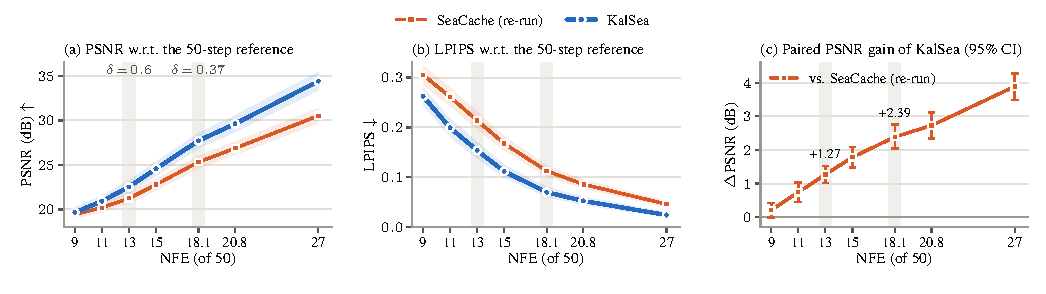
\includegraphics[width=\textwidth]{kalsea_fidelity.pdf}
  \caption[KalSea: fidelity versus compute]{Fidelity versus compute on FLUX.1-dev (DrawBench, 200 held-out prompts). (a) PSNR and (b) LPIPS with respect to the 50-step reference versus the mean NFE; the SEA-gate threshold $\delta\in\{0.2,0.3,0.37,0.5,0.6,0.8,1.0\}$, shared by all methods, sets the budget. All methods share code, seeds and hardware. Lines: means over prompts; shaded: 95\% bootstrap CIs. (c) Paired PSNR gain of KalSea over SeaCache with 95\% CIs.}
  \label{fig:kalsea-fidelity}
\end{figure}

\paragraph{Text-to-video.} We apply KalSea with the per-element filter to HunyuanVideo and Wan2.1-1.3B at SeaCache's two budgets (\cref{tab:kalsea-video}); on Wan2.1 (UniPC, classifier-free guidance) PCGS replays the solver. Because SeaCache's released HunyuanVideo script gates on a stale noise level near one, every gated method reads the sampler's noise level, with $\delta$ set for 24.0 and 16.0 NFE. Our re-run of SeaCache then reproduces its published result at 24 NFE (32.43 vs.\ 32.39\,dB) but not at 16.4 (24.53\,dB at 16.0 vs.\ 26.46\,dB; its released gate gives 20.52\,dB), so the table reports the re-run for HunyuanVideo. There, KalSea improves on SeaCache by 3.17\,dB $[2.99,3.35]$ at 24 NFE and by 1.92\,dB $[1.70,2.14]$ at 16 NFE (better on 90\% and 72\% of the prompts), with better SSIM and LPIPS. On Wan2.1 it exceeds SeaCache's published results by 5.07 and 2.07\,dB at 24 and 17 NFE; in our setup the paired gains are 2.27\,dB $[2.13,2.42]$ and 0.33\,dB $[0.16,0.49]$, the latter with clearly better SSIM ($+0.023$) and LPIPS ($-0.029$). Part of the distance to the published Wan2.1 numbers therefore comes from the setup (our clips have 65 frames).

\begin{table}[t]
  \centering
  \scriptsize
  \setlength{\tabcolsep}{3pt}
  \caption[KalSea on HunyuanVideo and Wan2.1]{Text-to-video results (944 VBench prompts, 65 frames, fidelity to the 50-step output). $^\dagger$Published by SeaCache (other GPUs); NFE $=50\times$TFLOPs/TFLOPs of the full run. $^\S$Our re-run of SeaCache's released code with the corrected gate (same code, seeds and GPUs as KalSea). Lat.: s/video on one B200, measured by us ($^*$SeaCache's method in our code at the NFE of KalSea).}
  \label{tab:kalsea-video}
  \begin{tabular}{@{}lcccccc@{\hspace{8pt}}cccccc@{}}
    \toprule
    & \multicolumn{6}{c}{HunyuanVideo, $480\times640$, 65 frames} & \multicolumn{6}{c}{Wan2.1 1.3B, $832\times480$, 65 frames} \\
    \cmidrule(r){2-7}\cmidrule(l){8-13}
    Method & NFE & TFLOPs & Lat. & PSNR$\uparrow$ & SSIM$\uparrow$ & LPIPS$\downarrow$ & NFE & TFLOPs & Lat. & PSNR$\uparrow$ & SSIM$\uparrow$ & LPIPS$\downarrow$ \\
    \midrule
    Reference (50 steps) & 50 & 14043 & 74.5 & -- & -- & -- & 50 & 6649 & 52.0 & -- & -- & -- \\
    \midrule
    \multicolumn{13}{@{}l}{\emph{$\approx$50\% budget (24--26 NFE)}} \\
    Fewer steps$^\dagger$ & 25.0 & 7019 & 39.9 & 19.97 & 0.731 & 0.263 & -- & -- & -- & -- & -- & -- \\
    TeaCache$^\dagger$ & 24.9 & 6994 & 40.2 & 23.40 & 0.805 & 0.133 & 25.0 & 3324 & 27.6 & 20.84 & 0.721 & 0.171 \\
    TaylorSeer$^\dagger$ & 26.0 & 7299 & 43.3 & 24.14 & 0.820 & 0.152 & 25.5 & 3391 & 29.1 & 16.15 & 0.543 & 0.336 \\
    SeaCache & 24.0$^\S$ & 6744 & 38.4 & 32.43 & 0.929 & 0.048 & 24.0$^\dagger$ & 3191 & 26.1$^*$ & 26.60 & 0.873 & 0.075 \\
    \textbf{KalSea} & 24.0 & 6745 & 38.6 & \textbf{35.60} & \textbf{0.951} & \textbf{0.028} & 24.0 & 3193 & 26.5 & \textbf{31.67} & \textbf{0.953} & \textbf{0.020} \\
    \midrule
    \multicolumn{13}{@{}l}{\emph{$\approx$30\% budget (15--18 NFE)}} \\
    Fewer steps$^\dagger$ & 15.0 & 4211 & 25.9 & 17.49 & 0.662 & 0.371 & -- & -- & -- & -- & -- & -- \\
    TeaCache$^\dagger$ & 17.1 & 4794 & 28.9 & 20.42 & 0.734 & 0.172 & 18.0 & 2393 & 20.6 & 18.88 & 0.645 & 0.245 \\
    TaylorSeer$^\dagger$ & 18.0 & 5053 & 32.6 & 20.42 & 0.733 & 0.242 & 18.0 & 2393 & 20.9 & 14.18 & 0.453 & 0.455 \\
    SeaCache & 16.0$^\S$ & 4498 & 27.4 & 24.53 & 0.813 & 0.155 & 17.0$^\dagger$ & 2261 & 19.1$^*$ & 21.78 & 0.740 & 0.170 \\
    \textbf{KalSea} & 16.0 & 4499 & 27.5 & \textbf{26.45} & \textbf{0.846} & \textbf{0.117} & 17.0 & 2263 & 19.4 & \textbf{23.85} & \textbf{0.851} & \textbf{0.090} \\
    \bottomrule
  \end{tabular}
\end{table}

\paragraph{Qualitative results.} \Cref{fig:kalsea-qual} shows one example per model at the lower budget, chosen by a fixed rule: among the prompts on which SeaCache and KalSea computed identical steps, the one whose PSNR gain of KalSea over SeaCache is closest to the upper quartile. SeaCache alters details that KalSea keeps, such as the street lamp added at the top right of the FLUX.1-dev image.

\begin{figure}[t]
  \centering
  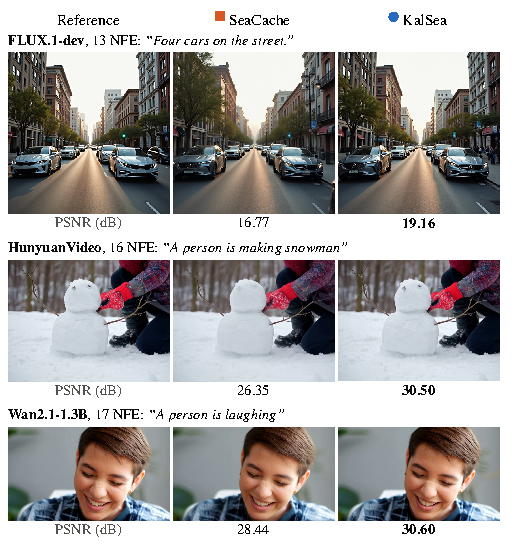
\includegraphics[width=0.9\textwidth]{kalsea_qualitative.pdf}
  \caption[KalSea: qualitative comparison]{One example per model at its lower budget (reference, SeaCache, KalSea): FLUX.1-dev ($\delta=0.6$, 13 NFE, ``Four cars on the street.'', PSNR 16.77 vs.\ 19.16\,dB), HunyuanVideo ($\delta=0.48$, 16 NFE, ``A person is making snowman'', 26.35 vs.\ 30.50\,dB) and Wan2.1-1.3B ($\delta=0.35$, 17 NFE, ``A person is laughing'', 28.44 vs.\ 30.60\,dB); video: frame 32 of 65.}
  \label{fig:kalsea-qual}
\end{figure}

\subsection{Ablations}\label{sec:kalsea-ablations}
\Cref{tab:kalsea-ablation} reports paired PSNR differences to KalSea at $\delta=0.3$ (20.8 NFE) and $\delta=0.6$ (13 NFE); differences below 0.1\,dB are within run-to-run noise.

\begin{table}[t]
  \centering
  \small
  \caption[KalSea ablations]{Ablations (FLUX.1-dev, DrawBench-200, held out). First row: PSNR of KalSea; other rows: paired PSNR difference to KalSea (dB, 95\% bootstrap CI). All rows share the SEA gate and threshold, with NFE within 0.06 (0.00) of KalSea at $\delta=0.3$ ($0.6$).}
  \label{tab:kalsea-ablation}
  \begin{tabular}{@{}lcc@{}}
    \toprule
    Variant & 20.8 NFE ($\delta=0.3$) & 13 NFE ($\delta=0.6$) \\
    \midrule
    KalSea (Kalman + PCGS) & 29.62\,dB & 22.53\,dB \\
    \midrule
    \multicolumn{3}{@{}l}{\emph{(a) Filler on skipped steps, no correction}} \\
    Reuse (SeaCache) & $-2.73$ $[-3.12,-2.34]$ & $-1.27$ $[-1.52,-1.02]$ \\
    Linear extrapolation & $-1.11$ $[-1.34,-0.89]$ & $-0.73$ $[-0.92,-0.54]$ \\
    Kalman (KalSea w/o PCGS) & $-0.83$ $[-1.02,-0.63]$ & $-0.61$ $[-0.76,-0.48]$ \\
    \multicolumn{3}{@{}l}{\emph{(b) Correction of the Kalman forecast}} \\
    Filter state only & $-0.86$ $[-1.06,-0.68]$ & $-0.63$ $[-0.78,-0.50]$ \\
    Linear interpolation & $+0.14$ $[+0.04,+0.25]$ & $+0.00$ $[-0.05,+0.06]$ \\
    Forecast + lin.\ innov. & $+0.14$ $[+0.04,+0.25]$ & $+0.02$ $[-0.03,+0.07]$ \\
    Batched re-integration & $-0.22$ $[-0.34,-0.09]$ & $-0.06$ $[-0.13,+0.01]$ \\
    No gate refresh & $+0.03$ $[-0.04,+0.10]$ & $+0.01$ $[-0.01,+0.03]$ \\
    \multicolumn{3}{@{}l}{\emph{(c) Other forecaster, with PCGS}} \\
    Per-element filter & $+0.01$ $[-0.15,+0.14]$ & $-0.01$ $[-0.15,+0.13]$ \\
    Damping $\tau=0.1$ & $-0.08$ $[-0.29,+0.12]$ & $+0.05$ $[-0.11,+0.22]$ \\
    Calibration-free & $-0.02$ $[-0.11,+0.08]$ & $+0.02$ $[-0.13,+0.17]$ \\
    \multicolumn{3}{@{}l}{\emph{(d) PCGS on other fillers}} \\
    Reuse + PCGS & $-1.03$ $[-1.39,-0.67]$ & $-0.53$ $[-0.76,-0.29]$ \\
    Linear extrap.\ + PCGS & $+0.04$ $[-0.08,+0.16]$ & $+0.07$ $[-0.05,+0.18]$ \\
    \bottomrule
  \end{tabular}
\end{table}

\paragraph{Anatomy of the corrector.} Without PCGS, PSNR drops by 0.83 and 0.61\,dB (Kalman row). Across budgets the predictor alone loses its advantage over reuse as gaps grow, while PCGS improves on it at every budget. The gain comes from re-integrating the latent: feeding the smoothed residuals only into the filter state is no better than no correction ($-0.86$ vs.\ $-0.83$\,dB at 20.8 NFE). Simpler gain shapes, such as a linear interpolation from $r_a$ to $r_b$, do as well as the RTS gains. The batched re-integration on the stored inputs $h^{\mathrm{in}}_i$ loses 0.22\,dB $[0.09,0.34]$ at 20.8 NFE, and the gate refresh has no measurable effect.

\paragraph{Other forecasters and fillers.} With PCGS, the forecaster's parametrisation hardly matters: the per-element filter, the damping $\tau=0.1$ of SpecKCast and a calibration-free filter all stay within 0.1\,dB of KalSea, so the frequency decomposition is unnecessary for the residual and the per-element filter is used for video. Nor is PCGS tied to a Kalman forecaster: it improves reuse by 1.69 and 0.74\,dB and linear extrapolation by 1.15 and 0.80\,dB; linear extrapolation with PCGS then ties KalSea, while reuse with PCGS stays 1.03 and 0.53\,dB below.

\subsection{Limitations}
Matched NFE is not matched latency: PCGS adds output-layer evaluations and 0.02\,GiB over KalSea w/o PCGS, and the filter adds element-wise work, so at equal NFE KalSea is 3--5\% slower than SeaCache on FLUX.1-dev and at most 1.4\% on video. The metrics measure fidelity to the 50-step sampler, which is the goal of a cache, not sample quality. The image results cover a single model. On Wan2.1 the same-setup PSNR gain is only 0.33\,dB at 17 NFE and negative at 10 NFE on 20 prompts. Finally, PCGS attaches the residual of the uncorrected latent to the corrected one, which is accurate only for small corrections; with gaps of up to twelve steps its gain is modest (0.31\,dB at 9 NFE).

%% ------------------------------------------------------------------------------------------------
\section{Comparison of ReSPect and KalSea}\label{sec:kalsea-compare}

\Cref{tab:kalsea-compare} compares the two methods of this project conceptually. Both use the same SEA gate and both forecast the block-stack residual rather than the hidden state. They differ in the forecaster (a global regression versus a recursive state-space filter) and, more fundamentally, in the loop: ReSPect predicts each skipped run from the past and never revisits it, whereas KalSea's state-space model provides the covariances needed to smooth the run once the next step has been observed, and PCGS re-integrates it.

\begin{table}[t]
  \centering
  \small
  \caption[Conceptual comparison of ReSPect and KalSea]{Conceptual comparison of the two methods developed in this project.}
  \label{tab:kalsea-compare}
  \begin{tabularx}{\textwidth}{@{}l>{\raggedright\arraybackslash}X>{\raggedright\arraybackslash}X@{}}
    \toprule
    & ReSPect & KalSea \\
    \midrule
    Gate (when) & SEA gate, reference refreshed every step & SEA gate (unchanged), live noise level, refreshed after correction \\
    Filler (what) & Ridge Chebyshev ($M{=}4$) + first-order Taylor, $w{=}0.5$ & Damped-trend Kalman filter (DCT bands or per element) \\
    Target & block-stack residual & block-stack residual \\
    Loop & open: past runs never corrected & closed: PCGS smooths and re-integrates every gap \\
    Theory & skip-length-independent Chebyshev bound; analytic blend and warm-up & RTS smoother gain in closed form; first-order optimal re-integration \\
    Extra cost & 1.7--4.3\% wall clock over reuse & one $\Emb$ + $\Out$ per skipped step; 3--5\% (images), $\le$1.4\% (video) over SeaCache \\
    State & $K$ residuals + $(M{+}1)\times F$ coefficients & 2 values per element + small covariances; gap buffer \\
    Hyper-parameters & $M,K,\lambda,w$, warm-up (fixed by analysis) & $\tau{=}0.5$, $R{=}10^{-3}$; PCGS adds none \\
    \bottomrule
  \end{tabularx}
\end{table}

A numerical comparison is possible on FLUX.1-dev, where both studies use the same model, resolution, step count, guidance and DrawBench-200 prompts, at matched NFE:
\begin{itemize}
  \item at 18.1 NFE, ReSPect ($\delta=0.37$) reaches 26.24\,dB (\cref{tab:respect-seacache}) and KalSea 27.72\,dB (\cref{tab:kalsea-flux});
  \item at 13 NFE, ReSPect ($\delta=0.6$) reaches 21.63\,dB (\cref{tab:respect-flux}) and KalSea 22.53\,dB.
\end{itemize}
The two studies were run in different harnesses, and their SeaCache re-runs differ slightly (25.45\,dB at 18.1 NFE in the ReSPect harness; about 25.33\,dB implied by KalSea's paired gain of 2.39\,dB), so the cross-study difference is indicative rather than a controlled comparison. Within each study the ordering is clear: ReSPect improves on SeaCache's reuse by $+0.79$\,dB at 18.1 NFE, and KalSea by $+2.39$\,dB, of which PCGS contributes $0.81$\,dB. The ablations of \cref{tab:kalsea-ablation} also explain why the two methods are complementary rather than competing: PCGS improved every filler on which it was tested (reuse, linear extrapolation and the Kalman forecast), and simple gain shapes such as a linear interpolation of the innovation worked as well as the RTS gains, so the closed loop of KalSea could in principle also be wrapped around ReSPect's forecaster; this combination has not been evaluated yet.
